\documentclass[tikz,border=10pt]{standalone}
\begin{document}
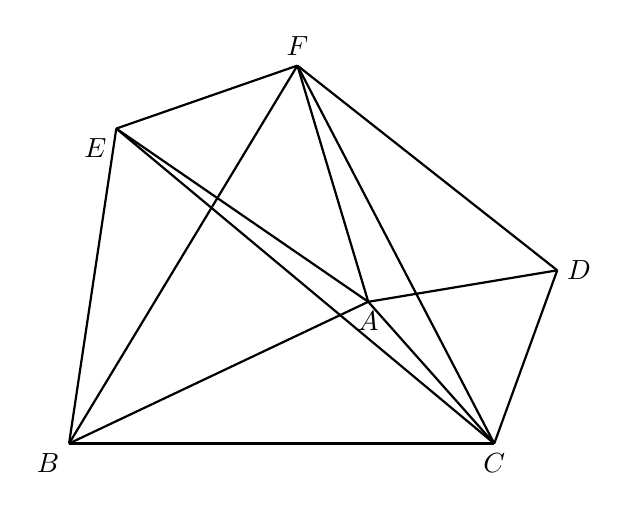
\begin{tikzpicture}[scale=1]
  \coordinate (A) at (4.2,1.8);
  \coordinate (B) at (0.4,0);
  \coordinate (C) at (5.8,0);
  \coordinate (D) at (6.6,2.2);
  \coordinate (E) at (1.0,4.0);
  \coordinate (F) at (3.3,4.8);

  \draw[thick] (A) -- (B);
  \draw[thick] (A) -- (C);
  \draw[thick] (A) -- (D);
  \draw[thick] (A) -- (E);
  \draw[thick] (A) -- (F);
  \draw[thick] (B) -- (C);
  \draw[thick] (B) -- (E);
  \draw[thick] (B) -- (F);
  \draw[thick] (C) -- (D);
  \draw[thick] (C) -- (E);
  \draw[thick] (C) -- (F);
  \draw[thick] (D) -- (F);
  \draw[thick] (E) -- (F);

  \node[below left] at (B) {$B$};
  \node[below] at (C) {$C$};
  \node[below] at (A) {$A$};
  \node[right] at (D) {$D$};
  \node[below left] at (E) {$E$};
  \node[above] at (F) {$F$};
\end{tikzpicture}
\end{document}
